Le principe du \game est le suivant : on dispose au départ d'un nombre $\nbAllumettes$ non nul d'allumettes
% IL EST IMPORTANT DE SPECIFIER QUE LE NB D'ALLUMETTES EST NON NUL CAR NOTRE DEF DE 0_PERD NE DEFINIT CETTE NOTION QUE POUR t>0 !!!
et un nombre $\nbJoueurs$ de joueurs peuvent prendre $1$ ou plusieurs allumette(s). Le joueur qui perd est celui qui, le premier, ne peut plus prendre d'allumette.\footnote{Il existe différentes variantes de ce jeu, notamment en faisant varier les nombres d'allumettes et de joueurs, mais également en faisant varier les actions possibles ou en introduisant des contraintes (par exemple, on ne peut pas prendre le même nombre d'allumettes que le joueur précédent).} Le nombre de tours de jeu possibles est au plus égal à celui des allumettes (à minima, chaque joueur ne prend à chaque tour qu'une seule allumette). Ainsi, l'ensemble des indices des tours possibles est $\turnsSet = \{ 0, ..., \nbAllumettes \}$ où $0$ est l'indice de l'état initial. De même, l'ensemble des nombres possibles d'allumettes encore disponibles est $\matchesSet = \{ 0, 1, ..., \nbAllumettes \}$.

Afin de simplifier au maximum le langage utilisé, nous modélisons ici une variante où $\nbAllumettes = 4$ et $\nbJoueurs = 2$. Les joueurs sont notés $0$ et $1$ et c'est au tour de $0$ de jouer au tour $t$ ssi $\turn{t}$ est vrai (considérant que si ce n'est pas le tour de $0$ alors c'est celui de $1$). De plus, $\rest{t}{n}$ est vrai ssi au tour $t$ il reste $n$ allumettes.

Ainsi, l'état initial du jeu est le suivant : 
\begin{gather}
\rest{0}{\nbAllumettes} \land \turn{0}
\label{eq:initialState}
\end{gather}
indiquant qu'au tour $0$ il y a encore $\nbAllumettes$ de disponible et que c'est au tour de $0$ de jouer.

Dans la version présentée ici du \game, on limite également le nombre des actions possibles à deux : un joueur peut prendre soit $1$ allumette, soit $2$ allumettes. Ainsi, $\takes{t}$ est vrai ssi un agent prend $2$ allumettes au tour $t$ (considérant ainsi que $\takes{t}$ est faux ssi il n'en prend qu'une). 

Ainsi :
\begin{align}
%\begin{split} TODO
\bigwedge_{\substack{t \in \turnsSet%\\
n \in \matchesSet%\\
n \geq 2}}
    \bigg ( & \Big ( \rest{t}{n} \land \takes{t} \limp%\\
    & \hspace{1.5cm}\rest{t+1}{n-2} \ \Big ) \; \land \\
    & \Big ( \rest{t}{n} \land \neg \takes{t} \limp %\\
    & \hspace{1.5cm}\rest{t+1}{n-1} \Big ) \bigg )
%\end{split}
\end{align}
capture le fait que si au tour $t$ il reste au moins $2$ allumettes et qu'un joueur en prend $2$ alors au tour suivant il en reste $2$ de moins, et que si il n'en prend qu'une alors au tour suivant il en reste $1$ de moins.

En revanche, si au tour $t$ il reste exactement $1$ allumette, alors nécessairement le joueur en prendra $1$ et il en restera $0$ au tour suivant :
\begin{gather}
\bigwedge_{t \in \turnsSet}
    \Big (\rest{t}{1} \limp \neg \takes{t} \land \rest{t+1}{0}\Big )
\end{gather}

Notre modèle spécifie ensuite que :
\begin{align}
& \bigwedge_{t \in \turnsSet}
    \bigvee_{n \in \matchesSet}
        \rest{t}{n} \\
& \bigwedge_{\substack{t \in \turnsSet\\ n1, n2 \in \matchesSet\\ n1 \neq n2}}
    \Big ( \rest{t}{n1} \limp \neg\rest{t}{n2} \Big )
\end{align}
La première formule stipule qu'à chaque tour $t$ il existe au moins un nombre $n$ d'allumettes restant, et la seconde que ce nombre est unique.

\begin{figure*}
\centering
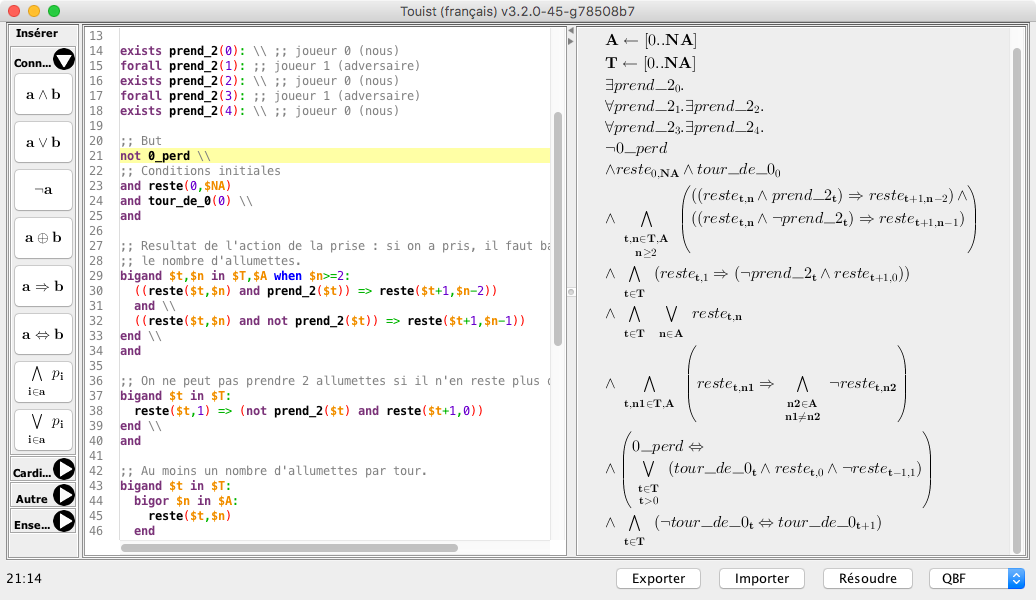
\includegraphics[width=0.9\textwidth]{Pictures/touistScreenshot}
\caption{Capture d'écran de \touist avec le \game. Le fichier est disponible à l'adresse \url{https://github.com/maelvalais/allumettes}}
\label{fig:touistScreenshot}
\end{figure*}

Il faut maintenant définir quand un joueur a perdu :
\begin{gather}
\begin{split}
\lost \lequiv \bigvee_{\substack{t \in \turnsSet\\ t > 0}} & \bigg ( \turn{t} \land \rest{t}{0} %\land \\
%    &  \Big ( \rest{t-1}{1} \lor \rest{t-1}{2} \Big 
\bigg )
\end{split}
\end{gather}
signifie que le joueur $0$ a perdu ssi il existe un tour $t$ où il reste $0$ allumettes alors qu'à l'instant d'avant il y en avait au moins une.

Finalement, à chaque tour $t$, ce n'est pas au joueur $0$ de jouer ssi c'est à lui de jouer au tour suivant :
\begin{gather}
\bigwedge_{t \in \turnsSet \setminus \{ \nbAllumettes \} } \Big (
    \neg \turn{t} \lequiv \turn{t+1}
\Big )
\label{eq:turnChange}
\end{gather}

